\section{Number of nodes vs. Tree Depth}
\label{nodes_vs_depth}

A simple measure of a tree's shape can be obtained by computing the number of
nodes as a function of depth. Consider the following trees:

\smallskip{}
\begin{tabular}{ccc}
\texttt{star} & \texttt{balanced} & \texttt{short\_leaves} \\
\hline \\
\includegraphics{nodes_vs_depth_1_svg.pdf} &
\includegraphics{nodes_vs_depth_2_svg.pdf} &
\includegraphics{nodes_vs_depth_3_svg.pdf}
\end{tabular}
\smallskip{}

\noindent{}they have the same depth and the same number of
leaves.  But their shapes are very different, and they tell different
biological stories. If we assume that they are clock-like (i.e., that the
mutation rate is constant over the whole tree), \texttt{star} shows an early
radiation, \texttt{short\_leaves} shows two stable lineages ending in
recent branching, while \texttt{balanced} shows branching spread over time.

The nodes-vs-depth graphs for these trees are as follows: \\
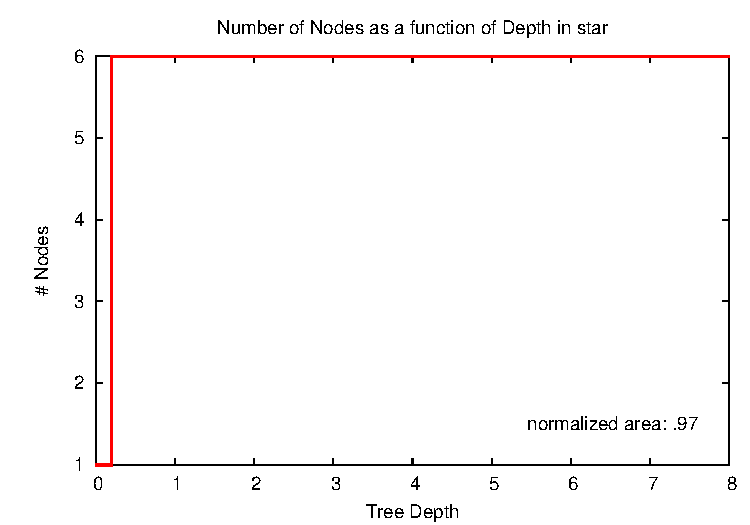
\includegraphics[width=12cm]{star.pdf} \\
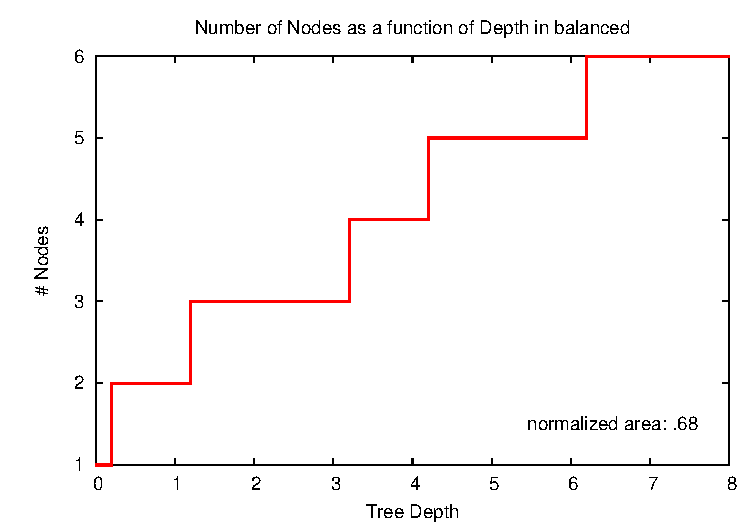
\includegraphics[width=12cm]{balanced.pdf} \\
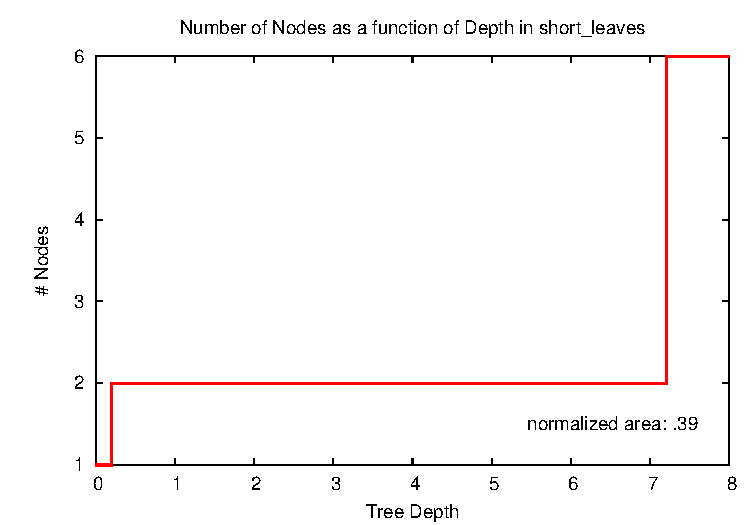
\includegraphics[width=12cm]{short_leaves.pdf} \\

The graphs show the (normalized) area under the curve: it is close to 1 for star-like trees, close to 0 for trees with very short leaves, and intermdiary for more balanced trees.

The images were made with the \texttt{nodes\_vs\_clades.sh} script (in
directory \texttt{src}), in the following way:
\begin{verbatim}
$ nodes_vs_clades.sh star 40
\end{verbatim}
where 40 is just the sampling density (how many points to take on the $x$
axis). The script uses \distance{} to get the tree's depth, \ed{} to sample the number of nodes at a given depth, and \nwindent{} to count the leaves, plus the usual \texttt{awk} and friends. The plot is done with gnuplot.
